\chapter{AHTR Modeling and Optimization Methodology}
In this chapter, I describe the modeling and optimization methodology of
\gls{ROLLO} \gls{AHTR} optimization for non-conventional geometries and parameters.
To wholly explore the design space enabled by additive manufacturing, the 
optimization tool should enable placement of fuel, moderation, and coolant material 
in any possible location, within physical limits. 
Since exploration of non-conventional geometries and parameters has barely been
attempted (previous attempts described in Section \ref{sec:lit-review-reactor-arbitrary}), 
this dissertation attempts a first go at beginning to explore the large design space.  
The work done for this dissertation is only an intermediate step towards developing 
a truly arbitrary geometry expression. 

%In the subsequent sections, I will define the optimization problem, describe the 
%AHTR geometries . 
%Then, I will describe the software used to model them and the specific models. 

\section{Optimization Problem Definition}
\label{sec:opt-problem}
In an effort towards optimizing reactor design for non-conventional geometries 
and parameters.
I chose to vary the following \gls{AHTR} parameters: 
\begin{itemize}
    \item \gls{TRISO} particle packing fraction distribution, 
    $\rho_{TRISO}(\vec{r})$
    \item Total fuel packing fraction
    \item \gls{FLiBe} coolant channel shape 
\end{itemize} 
The TRISO packing fraction distribution variation enables exploration of how 
heterogenous fuel distributions impact reactor performance.
In Chapter \ref{chap:fhr-benchmark}, the results demonstrated that increased fuel 
packing does not always correspond with increased $k_{eff}$ due to self-shielding
effects. 
Varying total fuel packing fraction and TRISO distribution synergistically enables exploration of
how heterogenous TRISO distribution could minimize self-shielding and in turn reduce the fuel 
required for a reactor design. 
The FliBe coolant channel shape variation enables exploration of how non-uniform 
channel shapes impact reactor performance. 

I selected three key \gls{AHTR} optimization objectives that address contrasting reactor 
core qualities. 
Table \ref{tab:objectives} describes each objective, how I quantified them, and the motivation.
\begin{table}[]
    \centering
    \onehalfspacing
    \caption{\acrfull{ROLLO} optimization problem objectives with their quantification 
    descriptions, and motivation.}
	\label{tab:objectives}
    \footnotesize
    \begin{tabular}{p{4cm}p{5cm}p{5cm}}
    \hline 
    \textbf{Objective}& \textbf{Quantification}& \textbf{Motivation} \\
    \hline
    Minimize fuel amount & Minimize total fuel packing fraction & Cost savings, Non-proliferation \\ 
    \hline
    Maximize heat transfer & Minimize maximum temperature & Enable system to perform at a higher power with minimized thermal stress \\
    \hline
    Minimize power peaking & Minimize power peaking factor normalized by fuel distribution & Efficient fuel utilization, longer core life, safety\\
    \hline
    \end{tabular}
\end{table}
I will vary the described parameters in the \gls{AHTR} plank and \gls{AHTR} one-third assembly 
geometries to optimize the described objectives. 
The plank optimization acts as a preliminary study to inform the more complex \gls{AHTR} one-third
assembly optimization setup. 
In the next section, I will describe both geometries. 

\section{AHTR Geometry for Optimization Problem}
The optimization process is applied to both the \gls{AHTR} plank and \gls{AHTR} one-third
assembly geometries.
The geometries are adapted from the \gls{AHTR} design in the \gls{FHR} benchmark,
outlined in Chapter \ref{chap:fhr-benchmark}.
The main differences occur in the fuel plank region (see Figure \ref{fig:ahtr-fuel-assembly}). 
In the \gls{FHR} benchmark, the TRISO particles are arranged in rectangular lattices within
two fuel stripes in the plank. 
For the optimization problem, I instead discretized each plank into ten cells with random 
TRISO packing and an individually controlled packing fraction. 
I also omit the graphite spacers. 

\subsection{AHTR Plank Geometry}
\label{sec:ahtr-plank-geometry}
The \gls{AHTR} plank is a single graphite fuel plank model from the \gls{AHTR} design (Figure 
\ref{fig:ahtr-fuel-assembly}). 
I modified the fuel plank to be straightened with perpendicular sides, instead 
of slanted as in Figure \ref{fig:ahtr-fuel-plank}, for ease of modeling. 
The original slanted \gls{AHTR} geometry will be used for the complex one-third assembly 
optimization setup. 
Figure \ref{fig:straightened_plank} illustrates the straightened fuel plank with 
ten fuel cells with random \gls{TRISO} packing.
\begin{figure}[]
    \centering
    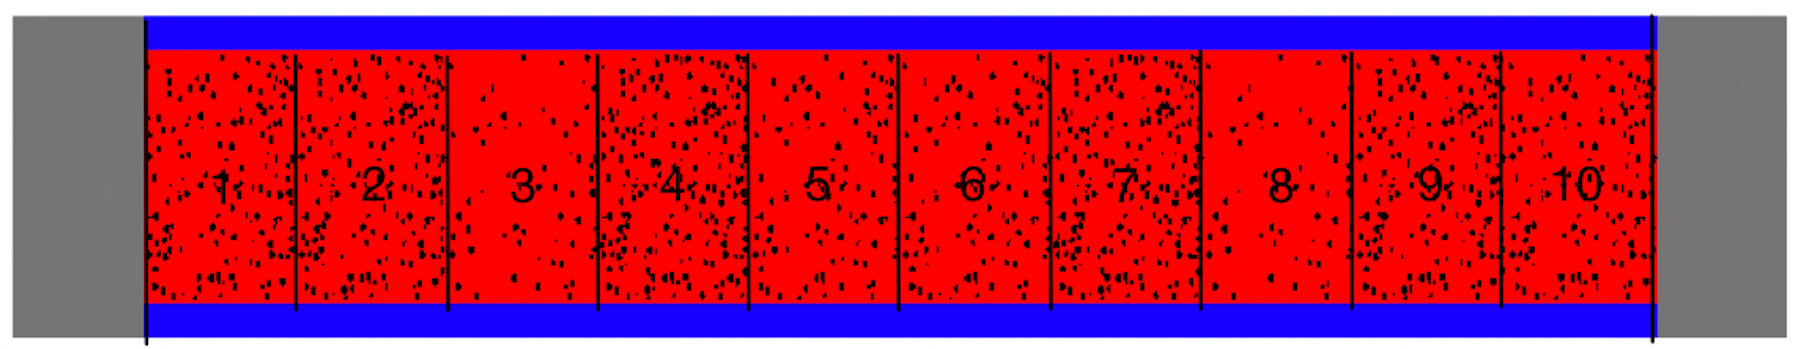
\includegraphics[width=0.85\linewidth]{straightened_plank.png}
    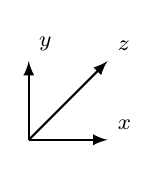
\begin{tikzpicture}
        \draw[ thick,-latex] (0,0) -- (1,0) node[anchor=south west] {$x$};
        \draw[ thick,-latex] (0,0) -- (0,1) node[anchor=south west] {$y$};
        \draw[ thick,-latex] (0,0) -- (1,1) node[anchor=south west] {$z$};
       \tkzText[above](-0.3,-0.7){}
       \end{tikzpicture} 
    \raggedright
    \resizebox{0.3\textwidth}{!}{
        \hspace{1cm}
        \fbox{\begin{tabular}{ll}
            \textcolor{fhrblue}{$\blacksquare$} & FLiBe \\
            \textcolor{fhrgrey}{$\blacksquare$} & Graphite (Structure)\\
            \textcolor{fhrred}{$\blacksquare$} & Graphite (Fuel Plank) \\
            \textcolor{fhrblack}{$\blacksquare$} & TRISO particle 

            \end{tabular}}}
    \caption{Straightened \acrfull{AHTR} fuel plank with 10 fuel cells with random 
    TRISO packing. Original slanted fuel planks can be seen in Figures 
    \ref{fig:ahtr-fuel-assembly} and \ref{fig:ahtr-fuel-plank}.}
    \label{fig:straightened_plank}
\end{figure}
The plank has $27.1 \times 3.25 \times 1.85\ cm^3$ dimensions with reflective 
boundary conditions.

I used the same materials as in the \gls{FHR} benchmark (Chapter \ref{chap:fhr-benchmark}), 
except that I homogenized each \gls{TRISO} particle's four outer layers: 
porous carbon buffer, inner pyrolytic carbon, silicon carbide layer, and the 
outer pyrolytic carbon. 
The \gls{TRISO} particle dimensions remain the same.
Table \ref{tab:keff_triso} reports OpenMC's reported $k_{eff}$ for this original 
straightened \gls{AHTR} configuration with and without the outer layer \gls{TRISO} 
homogenization.
\begin{table}[]
    \centering
    \onehalfspacing
    \caption{Straightened \acrfull{AHTR} fuel plank $k_{eff}$ for case with 
    no \gls{TRISO} homogenization and case with homogenization of the four outer 
    layers. Both simulations were run on one BlueWaters XE Node.}
	\label{tab:keff_triso}
    \footnotesize
    \begin{tabular}{llc}
    \hline 
    \textbf{TRISO Homogenization}& \textbf{$k_{eff}$} & \textbf{Simulation time [s]}  \\
    \hline 
    None & $1.38548 \pm 0.00124$ & 233\\ 
    Four outer layers & $1.38625 \pm 0.00109$ & 168\\ 
    \hline
    \end{tabular}
\end{table}
The \gls{TRISO} particle outer four-layer homogenization resulted in a $30\%$ 
speed-up without compromising accuracy with $k_{eff}$ values within each 
other's uncertainty.

% coolant channel shape variation

\subsection{AHTR One-Third Assembly Geometry}
The \gls{AHTR} one-third assembly is one-diamond shape sector of the \gls{AHTR} assembly and
contains six fuel planks.
Each graphite plank has graphite buffers and ten rectangular prism fuel cells 
with random TRISO packing and individually controlled packing fraction. 
Figure \ref{fig:ahtr_assembly} shows the one-third \gls{AHTR} assembly with 10 x 6 fuel cells with 
random \gls{TRISO} packing.
\begin{figure}[]
    \centering
    \begin{subfigure}{.7\textwidth}
    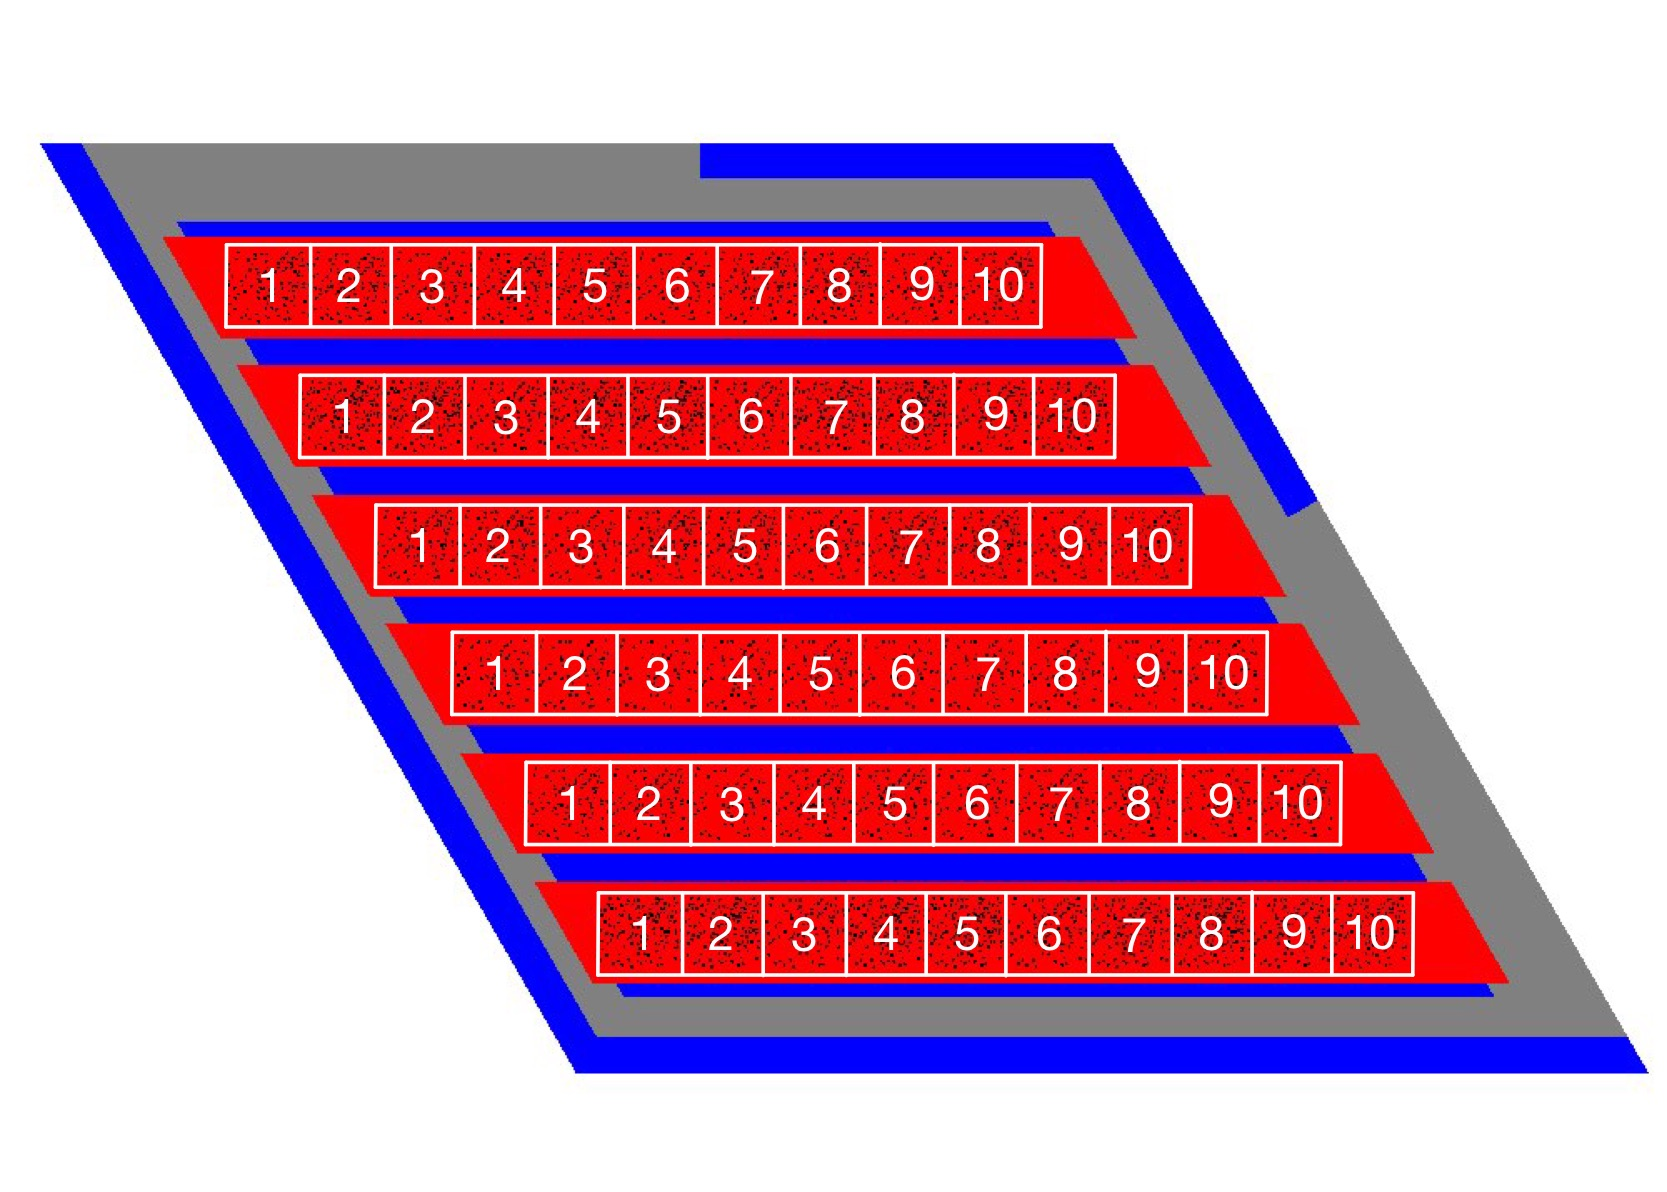
\includegraphics[width=\linewidth]{ahtr_assembly.png}
    \end{subfigure}%
    \begin{subfigure}{.3\textwidth}
        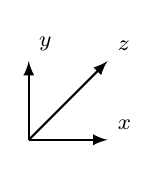
\begin{tikzpicture}
            \draw[ thick,-latex] (0,0) -- (1,0) node[anchor=south west] {$x$};
            \draw[ thick,-latex] (0,0) -- (0,1) node[anchor=south west] {$y$};
            \draw[ thick,-latex] (0,0) -- (1,1) node[anchor=south west] {$z$};
           \tkzText[above](-0.3,-0.7){}
        \end{tikzpicture} 
        \vspace{1cm}
        \fbox{\begin{tabular}{ll}
            \textcolor{fhrblue}{$\blacksquare$} & FLiBe \\
            \textcolor{fhrgrey}{$\blacksquare$} & Graphite (Structure)\\
            \textcolor{fhrred}{$\blacksquare$} & Graphite (Fuel Plank) \\
            \textcolor{fhrblack}{$\blacksquare$} & TRISO particle 
            \end{tabular}}
    \end{subfigure}
    \caption{\gls{AHTR} assembly with 10 fuel cells in each graphite plank with random 
    TRISO packing. Original \gls{FHR} benchmark fuel assembly with fuel stripes can be seen in 
    Figure \ref{fig:ahtr-fuel-assembly}.}
    \label{fig:ahtr_assembly}
\end{figure}
The assembly model also uses the \gls{TRISO} particle outer four layer homogenization described 
in Section \ref{sec:ahtr-plank-geometry}.

% coolant channel shape variation

\section{AHTR Model Workflow}
\gls{ROLLO} drives the evolutionary algorithm optimization process. 
In the \gls{ROLLO} input file, I will define control variables for the genetic algorithm 
to vary. 
These control variables are values used to control the \gls{AHTR} parameters described in 
Section \ref{sec:opt-problem}.
These control variables will be input into templated nuclear software to model different 
AHTR geometries.
The software will then run the \gls{AHTR} models and calculate the optimization objective 
and constraint values. 
In this work, I use OpenMC \cite{romano_openmc:_2015} to model \gls{AHTR}'s neutronics 
and Moltres \cite{lindsay_introduction_2018} to model the \gls{AHTR}'s multi-physics. 
Details about the software can be found in Section \ref{sec:lit-review-modeling-software}.

In this section, I describe the \gls{AHTR} modeling workflow: from the AHTR geometry 
variation input parameters, to the OpenMC and Moltres models, and finally the 
output and constraint values. 
This corresponds to the \textit{evaluate population} orange blocks in Figure 
\ref{fig:genetic_alg_nuclear}'s genetic algorithm flow chart.
Figure \ref{fig:ahtr-model-flow} illustrates the modeling workflow. 
\begin{figure}[]
    \centering
    \begin{tikzpicture}[node distance=0.5cm]
        \tikzstyle{every node}=[font=\footnotesize]
        \node (1) [e72block] {\textit{Total PF}};
        \node (2) [b72block, right=of 1] {PF};
        \node (3) [e72block, above=of 2] {Input Parameters};
        \node (4) [e72block, below=of 1] {$\rho_{TRISO}(\vec{r})$};
        \node (5) [b72block, right=of 4] {a, b, c, d, e, f};
        \node (6) [e72block, below=of 4] {FliBE Coolant Channel Shape};
        \node (7) [b72block, right=of 6] {$r_{top}$, $r_{bot}$};
        \node (8) [o72block, right=of 2, xshift=0.8cm, yshift=0.5cm] {OpenMC Model};
        \node (9) [e72block, above=of 8] {Nuclear Software Models};
        \node (10) [o72block, right=of 5, xshift=0.8cm] {Group Constants};
        \node (11) [o72block, right=of 7, xshift=0.8cm, yshift=-0.5cm] {Moltres Model};
        \node (12) [b72block, right=of 8, xshift=0.8cm, yshift=0.8cm] {$k_{eff}$}; 
        \node (13) [e72block, above=of 12] {Constraints};
        \node (14) [e72block, below=of 12] {Objectives};
        \node (15) [b72block, below=of 14] {PF};
        \node (16) [b72block, below=of 15] {PPF};
        \node (17) [b72block, below=of 16] {$T_{max}$};
        \draw [arrow] (2) -- ([shift={(0cm,0cm)}]2.east) -- ([shift={(0cm,0cm)}]8.west);
        \draw [arrow] (5) -- ([shift={(0cm,0cm)}]5.east) -- ([shift={(0cm,0cm)}]8.west);
        \draw [arrow] (7) -- ([shift={(0cm,0cm)}]7.east) -- ([shift={(0cm,0cm)}]8.west);
        \draw [arrow] (7) -- ([shift={(0cm,0cm)}]7.east) -- ([shift={(0cm,0cm)}]11.west);
        \draw [arrow] (8) -- ([shift={(0cm,0cm)}]8.south) -- node[anchor=west] {generates} ([shift={(0cm,0cm)}]10.north);
        \draw [arrow] (10) -- ([shift={(0cm,0cm)}]10.south) -- node[anchor=west] {input into} ([shift={(0cm,0cm)}]11.north);
        \draw [arrow] (8) -- ([shift={(0cm,0cm)}]8.east) -- ([shift={(0cm,0cm)}]12.west);
        \draw [arrow] (8) -- ([shift={(0cm,0cm)}]8.east) -- ([shift={(0cm,0cm)}]15.west);
        \draw [arrow] (8) -- ([shift={(0cm,0cm)}]8.east) -- ([shift={(0cm,0cm)}]16.west);
        \draw [arrow] (11) -- ([shift={(0cm,0cm)}]11.east) -- ([shift={(0cm,0cm)}]17.west);
    \end{tikzpicture}
    \caption{\acrfull{AHTR} modeling workflow in ROLLO optimization.} 
    \label{fig:ahtr-model-flow}
\end{figure}

\subsection{Input Parameter Modeling}
\label{sec:input-parameter-modeling}
In this section, I describe how I modeled the \gls{AHTR} parameter variations: total fuel packing 
fraction, \gls{TRISO} particle packing fraction distribution, and \gls{FLiBe} coolant channel shape. 
For both the \gls{AHTR} plank and one-third assembly models, total fuel packing fraction parameter 
is a single numerical input.
I describe the other two parameters for both the \gls{AHTR} plank and one-third assembly. 

\subsubsection{Input Parameter Modeling: TRISO particle packing fraction distribution}
For both the \gls{AHTR} plank and one-third assembly, I utilize sine distributions to govern the 
\gls{TRISO} particle packing fraction distribution. 
Based on the sine distributions, the model calculates the packing fraction in each fuel cell, then use 
OpenMC's \texttt{pack\_spheres} function to randomly disperse the calculated packing fraction in each 
fuel cell. 
For the \gls{AHTR} plank, one sine distribution governs the \gls{TRISO} packing fraction distribution 
across the fuel plank's x-direction. 
For the \gls{AHTR} one-third assembly, two sine distributions govern the \gls{TRISO} packing fraction 
distribution across each fuel plank's x-direction, and the assembly's y-direction, respectively. 

For the \gls{AHTR} plank, a sine distribution governs the \gls{TRISO} particle packing fraction 
distribution across the ten fuel cells, illustrated in Figure \ref{fig:straightened_plank}:
\begin{align}
    PF(x) &= \left(a\cdot sin(b\cdot x + c) + 2\right) \cdot NF\\
    \intertext{where}
    PF &= \mbox{packing fraction } [-] \nonumber \\ 
    a &= \mbox{amplitude, peak deviation of the function from zero } [-] \nonumber \\
    b &= \mbox{angular frequency, rate of change of the function argument } [\frac{radians}{cm}] \nonumber \\
    c &= \mbox{phase, the position in its cycle the oscillation is at t = 0 } [radians]\nonumber \\
    x &= \mbox{midpoint value for each cell } [cm]\nonumber \\
    NF &= \mbox{normalization factor } [-]\nonumber
\end{align}
The sine distribution's coefficients, \textit{a b c}, are the control variables \gls{ROLLO} 
utilizes to control the TRISO packing fraction distribution in the plank.
Thus, \gls{ROLLO} will vary $a, b, c$ constants to find an optimal TRISO particle 
sine distribution. 
The normalization factor ensures the correct total packing fraction 
in the plank regardless the \gls{TRISO} particle distribution.

For example in a \gls{AHTR} plank with a 0.0979 total packing fraction, and packing fraction 
distribution of $PF(x) = \left(0.5\cdot sin(\frac{\pi}{3}\cdot x + \pi) + 2\right)  \cdot NF$, 
results in the following packing fractions for the ten cells: 0.103, 0.120, 
0.049, 0.138, 0.076, 0.081, 0.136, 0.048, 0.125, and 0.098. 
Figure \ref{fig:triso_distribution} shows this sine distribution, highlights 
the packing fraction at the respective midpoints, and displays the plank's x-y 
axis view with packing fraction varying based on this sine distribution. 
\begin{figure}[]
    \centering
    \makebox[\textwidth][c]{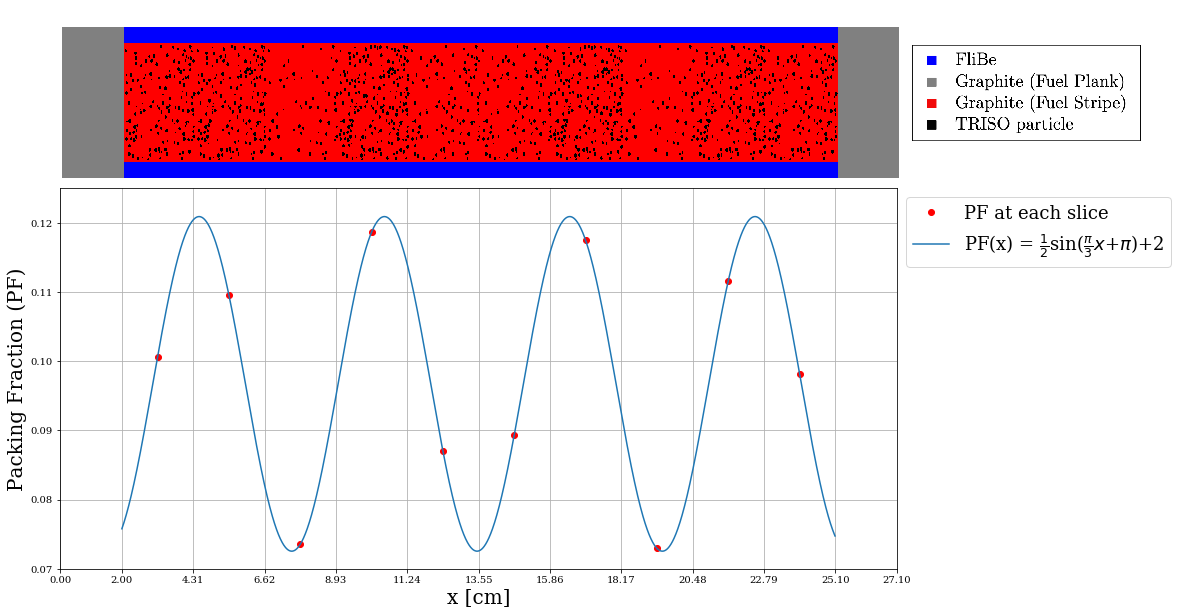
\includegraphics[width=1.1\linewidth]{triso_distribution_sine.png}} 
    \caption{Above: Straightened \acrfull{AHTR} fuel plank with varying \gls{TRISO} particle 
    distribution across ten cells based on the sine distribution. 
    Below: $PF(x) = (0.5\ sin(\frac{\pi}{3}x + \pi) + 2)  \times NF$ 
    sine distribution with red points indicating the packing fraction at each cell. }
    \label{fig:triso_distribution}
\end{figure}

For the \gls{AHTR} one-third assembly, two sine distributions govern the x and y direction
\gls{TRISO} particle packing fraction distributions in the 10 x 6 fuel cell shape, illustrated in 
Figure \ref{fig:ahtr_assembly}:
\begin{align}
    PF(x, y) &= \left(a\cdot sin(b\cdot x + c) + 2\right) 
    \cdot \left(d\cdot sin(e\cdot y + f) + 2\right) \cdot NF \\
    \intertext{where}
    PF &= \mbox{packing fraction } [-] \nonumber \\ 
    a, d &= \mbox{amplitude, peak deviation of the function from zero } [-] \nonumber \\
    b, e &= \mbox{angular frequency, rate of change of the function argument } [\frac{radians}{cm}] \nonumber \\
    c, f &= \mbox{phase, the position in its cycle the oscillation is at t = 0 } [radians]\nonumber \\
    x &= \mbox{midpoint value for each x-direction fuel cell } [cm]\nonumber \\
    y &= \mbox{midpoint value for fuel plank } [cm]\nonumber \\
    NF &= \mbox{normalization factor } [-]\nonumber
\end{align}
The sine distribution's coefficients, \textit{a b c d e f}, are the control variables \gls{ROLLO} 
utilizes to control the TRISO packing fraction distribution in the assembly.
Thus, \gls{ROLLO} will vary \textit{a b c d e f} constants to find an optimal TRISO particle 
distribution. 
The normalization factor ensures the correct total packing fraction 
in the plank regardless the \gls{TRISO} particle distribution.

For example in an \gls{AHTR} one-third assembly with a 0.1 total packing fraction, and packing 
fraction distribution of $PF(x, y) = \left(0.5\cdot sin(1\cdot x + 1) + 2\right) \cdot 
\left(0.7\cdot sin(1.5\cdot y + 2) + 2\right) \cdot NF$ results in the packing fraction 
distribution shown in Figure \ref{fig:ahtr-assem-triso-distr-squares}.
This corresponds to the one-third assembly with varying TRISO distribution in its fuel 
cells, shown in Figure \ref{fig:ahtr-assem-triso-distr}. 
\begin{figure}[]
    \centering
    \begin{subfigure}{0.49\textwidth}
        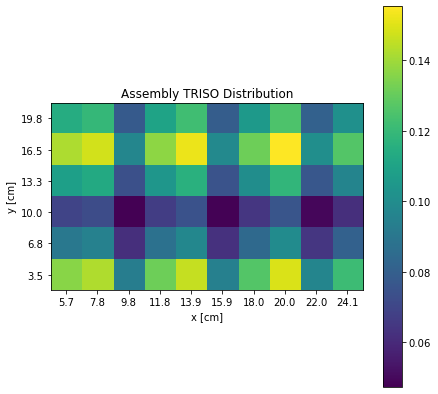
\includegraphics[width=\linewidth]{ahtr-assem-triso-distr-squares.png}
        \caption{}
        \label{fig:ahtr-assem-triso-distr-squares} 
    \end{subfigure}
    \begin{subfigure}{0.49\textwidth}
        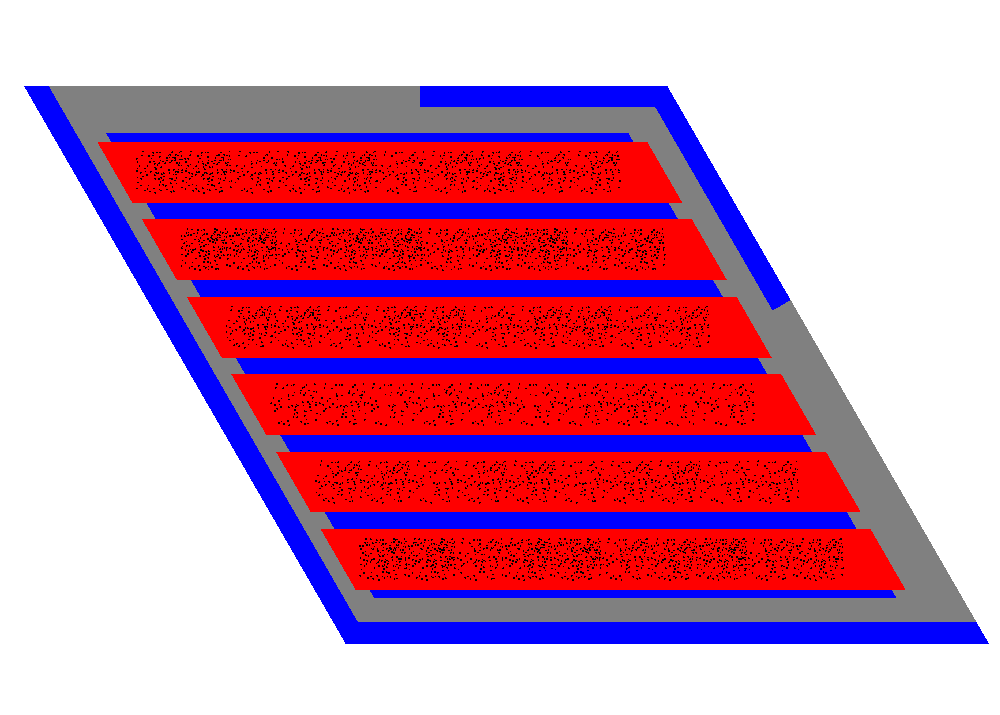
\includegraphics[width=\linewidth]{ahtr-assem-triso-distr.png}
        \raggedleft
        \resizebox{0.5\textwidth}{!}{
        \hspace{1cm}
        \fbox{\begin{tabular}{ll}
            \textcolor{fhrblue}{$\blacksquare$} & FLiBe \\
            \textcolor{fhrgrey}{$\blacksquare$} & Graphite (Structure) \\
            \textcolor{fhrred}{$\blacksquare$} & Graphite (Fuel Plank) \\
            \textcolor{fhrblack}{$\blacksquare$} & TRISO particle 
        \end{tabular}}}
        \caption{}
        \label{fig:ahtr-assem-triso-distr} 
    \end{subfigure}
    \caption{}
\end{figure}

\subsubsection{Input Parameter Modeling: FliBe Coolant Channel Shape}
I model the variation in coolant channel shape with a sinusoidal-like pattern.
I use cylinder surfaces in OpenMC, instead of a sinusoidal function. 
Creating complicated sinusoidal shapes in OpenMC requires the use of DAGMC, a CAD based tool, 
which is out of scope of the dissertation.
By varying the radius of the cylinder, the depth and frequency of the coolant channel shape 
minimics a sinusoidal-like pattern.
I vary the FliBE coolant channel shape while holding the total coolant area constant. 

For the \gls{AHTR} plank, $radius_{top}$ and $radius_{bot}$ variables control the coolant channel 
shape on the bottom and top FliBe channels. 
Figure \ref{fig:coolant-channel-shape} shows the \gls{AHTR} plank's coolant channel shape 
for $radius_{top} = 0.2$ and $radius_{bot} = 0.3$.
\begin{figure}[]
    \centering
        
\includegraphics[width=\linewidth]{coolant-channel-shape.png}
    \raggedright
    \resizebox{0.3\textwidth}{!}{
        \hspace{1cm}
        \fbox{\begin{tabular}{ll}
            \textcolor{fhrblue}{$\blacksquare$} & FLiBe Coolant\\
            \textcolor{fhrgrey}{$\blacksquare$} & Graphite (Structure) \\
            \textcolor{fhrred}{$\blacksquare$} & Graphite (Fuel Plank) \\
            \textcolor{fhrblack}{$\blacksquare$} & TRISO particle 
        \end{tabular}}}
    \caption{AHTR Fuel Plank with Coolant Shape Variation, $radius_{top} 
    = 0.2$ and $radius_{bot} = 0.3$.}  
    \label{fig:coolant-channel-shape}
\end{figure}
$radius_{top}$ and $radius_{bot}$ are the control variables \gls{ROLLO} 
utilizes to control the coolant channel shape in the \gls{AHTR} plank.
Thus, \gls{ROLLO} will vary $radius_{top}$ and $radius_{bot}$ to find an optimal coolant 
channel shape.

% Assembly COolant channel shape variation

\subsection{AHTR OpenMC and Moltres Models}
\label{sec:ahtr-moltres-hom}
The input parameter modeling outlined in the previous section are inputs into 
the OpenMC neutronics and Moltres multiphysucs models. 
In this section, I describe details and assumptions for the models. 

\subsubsection{AHTR OpenMC Model}
The OpenMC templated model accepts the following input parameters: total packing fraction, 
TRISO particle distribution, and FliBe coolant channel shapes, from \gls{ROLLO}.
The OpenMC model takes the input parameters and generates an \gls{AHTR} model with 
\gls{TRISO}-level fidelity. 
A separate OpenMC output file analyzes the results output from the OpenMC model and 
calculates the $k_{eff}$ constraint value and normalized power peaking factor output value.
Section \ref{sec:ahtr_slab_output} gives further description of calculation for 
each output and constraint parameter.
Figures \ref{fig:triso_distribution}, \ref{fig:ahtr-assem-triso-distr},
\ref{fig:coolant-channel-shape} are \gls{AHTR} model snapshots generated by OpenMC. 

\subsubsection{AHTR Moltres Group Constant Generation}
\label{sec:ahtr-moltres-group-constant-gen}
Unlike the OpenMC model, Moltres does not explicitly model each \gls{TRISO}
particle. 
This is because a TRISO-level fidelity mesh file is impractical and will result in an extremely 
long runtimes. 
Instead, Moltres relies on the OpenMC model to generate group constants data for the 
Moltres' multigroup neutron diffusion calculations. 
Previously, Moltres could only generate group constant data from Serpent 
\cite{leppanen_serpent_2014} or SCALE \cite{bucholz_scale:_1982} output files. 
I implemented functionality in Moltres for group constant data generation with 
OpenMC. 

To enable successful \gls{AHTR} Moltres simulations, I established suitable spatial and 
energy homogenization for group constant generation. 
These homogenizations preserve accuracy while maintaining an acceptable runtime.
For both the \gls{AHTR} plank and one-third assembly models, I used eight precursor groups 
and a four group energy structure derived by Gentry et al. \cite{gentry_development_2016} 
for \gls{AHTR} geometries. 
Table \ref{tab:energy_structures} defines the group boundaries. 
\begin{table}[]
    \centering
    \onehalfspacing
    \caption{4-group energy structures for \acrfull{AHTR} geometry 
    derived by \cite{gentry_development_2016}.}
	\label{tab:energy_structures}
    \footnotesize
    \begin{tabular}{lll}
    \hline
    \multicolumn{3}{c}{\textbf{Group Boundaries [MeV]}} \\ 
    \hline
    \textbf{Group $\#$}& \textbf{Upper Bound} & \textbf{Lower Bound}  \\
    \hline 
    1 & $2.0000\times 10^1$ & $9.1188\times 10^{-3}$ \\ 
    2 & $9.1188\times 10^{-3}$ & $2.9023\times 10^{-5}$\\
    3 & $2.9023\times 10^{-5}$ & $1.8554\times 10^{-6}$\\
    4 & $1.8554\times 10^{-6}$ & $1.0000\times 10^{-12}$\\
    \hline
    \end{tabular}
\end{table}

For spatial homogenization of the straightened \gls{AHTR} fuel plank, I used 
OpenMC's \textit{cell} domain type to compute multigroup cross sections for 
different \textit{cells}. 
I discretized the plank into 13 \textit{cells}: FLiBe, left graphite, right 
graphite, and ten fuel cells (each cell has a different packing fraction).
Figure \ref{fig:straightened_slab_mg} illustrates the \gls{AHTR} spatial 
homogenization for the OpenMC multigroup calculation. 
\begin{figure}[]
    \centering
    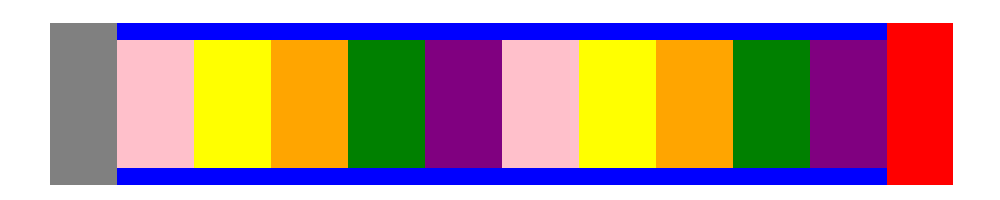
\includegraphics[width=\linewidth]{straightened_slab_mg.png}
    \raggedright
    \resizebox{0.5\textwidth}{!}{
        \hspace{1cm}
        \fbox{\begin{tabular}{llll}
            \textcolor{fhrblue}{$\blacksquare$} & FLiBe & 
            \textcolor{fhrgrey}{$\blacksquare$} & Left Graphite \\
            \textcolor{fhrred}{$\blacksquare$} & Right Graphite &
            \textcolor{fhrpink}{$\blacksquare$} & Fuel cell 1/6 \\
            \textcolor{fhryellow}{$\blacksquare$} & Fuel cell 2/7 &
            \textcolor{fhrorange}{$\blacksquare$} & Fuel cell 3/8 \\
            \textcolor{fhrgreen}{$\blacksquare$} & Fuel cell 4/9 &
            \textcolor{fhrpurple}{$\blacksquare$} & Fuel cell 5/10 \\
            \end{tabular}}}
    \caption{Straightened \acrfull{AHTR} fuel slab spatially discretized into 
    13 \textit{cells} for OpenMC multigroup calculation.}
    \label{fig:straightened_slab_mg}
\end{figure}

For spatial homogenization of the \gls{AHTR} one-third assembly... 
% include details about spatial homogenization for one-third assembly. 

To ensure that the spatial and energy homogenization preserves accuracy, I 
compared key neutronics parameters for the continuous OpenMC and multigroup 
Moltres simulations, for both the \gls{AHTR} plank and one-third assembly.
The results of the verification studies are described in Section 
\ref{sec:ahtr_model_verification}.

\subsubsection{AHTR Moltres Mesh Generation}
I wrote a python script that accepts the FliBe coolant channel shape input 
parameters and generates a geometry script file (\texttt{.geo}) based on the 
spatial homogenization outlined in Section \ref{sec:ahtr-moltres-hom}.
The AHTR geometry mesh is then generated from the geometry script file using 
Gmsh \cite{geuzaine_gmsh_2009}.
I used Gmsh's \textit{refine by splitting} functionality to refine the mesh. 

\subsubsection{AHTR Moltres Temperature Model}
\label{sec:ahtr-moltres-temperature-model}
The group constants and mesh file are inputs to the Moltres AHTR Steady-State 
Temperature Model.
The model first solves for the neutronics and uses that to solve for the \gls{AHTR}'s 
temperature distribution for a defined power. 
The temperature model assumes conductive heat transfer throughout the domain 
and heat removal by uniform salt flow in the coolant region. 
These assumptions ignore flow and turbulent effects that would most likely be 
present. 
However, an in-depth AHTR Moltres model that includes turbulence model is 
out of scope for this dissertation. 

Moltres solves the four-group diffusion equations (Equation \ref{eq:moltres-diffusion-equation}) 
as a steady-state eigenvalue problem to find $k_{eff}$ for the static AHTR slab model.
In the 2D cross-sectional AHTR Steady-State Temperature Model, I ignore the 
time-dependent and velocity-dependent terms from Moltres' temperature governing 
equation (Equation \ref{eq:moltres-temp}) since it is a steady-state model with
no moving fuel: 
\begin{align}
    - \nabla \cdot (k_i \nabla T) &= Q_i
\intertext{where:}
k_i &= \mbox{thermal conductivity of material i} \nonumber \\
T &= \mbox{temperature in the slab} \nonumber \\
Q_i &= \mbox{source or sink term in material i} \nonumber
\end{align} 
I use insulated temperature boundary conditions.  
Table \ref{tab:ahtr-thermal-conducitivity} shows the thermal conductivity values 
used for each AHTR slab material. 
% add citations
\begin{table}[]
    \centering
    \onehalfspacing
    \caption{AHTR Fuel Slab materials' thermal conductivity.}
	\label{tab:ahtr-thermal-conducitivity}
    \footnotesize
    \begin{tabular}{lp{4cm}l}
    \hline 
    \textbf{Material}& \textbf{Thermal Conductivity [$Wcm^{-1}K^{-1}$]}& \textbf{References} \\ 
    \hline 
    FliBE & 0.01 & \\
    Graphite  & 0.15 & \\
    Fuel  & 0.099 & \\
    \hline
    \end{tabular}
\end{table}

Equation \ref{eq:moltres-source-term} defines the fuel cells' fission source term.
Moltres' source term ($Q_f$) is defined by: 
\begin{align}
\label{eq:moltres-source-term}
    Q_f &= \sum_{g=1}^G \epsilon_{f,g}\Sigma_{f,g}\phi_g
\intertext{where} 
Q_f &= \mbox{source term } [\frac{MeV}{cm^3s}] \nonumber \\
G &= \mbox{number of discrete groups, g } [-] \nonumber \\
\epsilon_{f,g} &= \mbox{heat produced per fission } [MeV] \nonumber \\
\Sigma_{f,g} &= \mbox{macroscopic cross section for fission due to neutrons in group g } [\frac{1}{cm}] \nonumber \\
\phi_g &= \mbox{flux of neutrons in group g } [\frac{n}{cm^2s}]\nonumber
\end{align}

Equation \ref{eq:moltres-heat-removal} defines the heat removal from the AHTR 
fuel slab in the coolant areas: 
\begin{align}
    \label{eq:moltres-heat-removal}
    Q &= h \cdot (T(\vec{r})-T_{ref})
\intertext{where:}
Q &= \mbox{heat removal rate for 1cm thin slice of AHTR slab [W/cm]} \nonumber \\
h &= \mbox{heat transfer coefficient } [\frac{W}{cm \cdot K}] \nonumber \\
T(\vec{r}) &= \mbox{temperature at point $\vec{r}$ [K]} \nonumber \\
T_{ref} &= \mbox{reference temperature [K]} \nonumber
\end{align}

Table \ref{tab:heat-exchanger-constants} shows the values used for 
reference temperature and heat transfer coefficient for the convective 
heat transfer process.
\begin{table}[H]
    \centering
    \onehalfspacing
    \caption{AHTR Fuel Slab's heat transfer constants.}
	\label{tab:heat-exchanger-constants}
    \footnotesize
    \begin{tabular}{llll}
    \hline 
    \textbf{Constant}& \textbf{Value}& \textbf{Units} & \textbf{Notes} \\
    \hline 
    h & 990 & $\frac{W}{cm \cdot K}$ & Calculated in Eq. \ref{eq:calc-htc} \\
    $T_{ref}$ & 923 & K & AHTR Inlet Temperature \\ %cite ahtr 923K inlet temp 
    \hline
    \end{tabular}
\end{table} 
I calculated the heat transfer coefficient ($h$) using Equation \ref{eq:calc-htc} 
for the 1cm-thick AHTR $\Delta z$ slice with the following assumptions: 
\begin{itemize}
    \item it generates a constant amount of power, all of which is removed 
    by the coolant
    \item heat removal occurs at the coolant areas
    \item temperature increase per 1cm slice is constant from the inlet to the 
    outlet 
\end{itemize} 
\begin{align}
    \label{eq:calc-htc}
    h &= \frac{P_{dz}}{A_{coolant}} \div \frac{T_{total}}{H} \\
      &= \frac{1456 W}{23.1 * 0.5 * 2 cm^2} / (50 K / 550 cm) \nonumber \\
      &= 990 W cm^{-1}K^{-1} \nonumber 
\intertext{where:}
h &= \mbox{heat transfer coefficient } [\frac{W}{cm \cdot K}] \nonumber \\
P_{dz} &= \mbox{power produced in 1cm AHTR slab dz slice [$W$]}\nonumber \\
A_{coolant} &= \mbox{cross-sectional coolant area in AHTR slab [$cm^2$]} \nonumber \\
T_{total} &= \mbox{total temperature change from inlet to outlet [$K$]} \nonumber \\
H &= \mbox{AHTR height from inlet to outlet [$cm$]} \nonumber 
\end{align}
In the ROLLO optimization simulations, I vary the FliBE coolant channel shape. 
During the shape variation, I hold the coolant area constant. 
Therefore, the Moltres temperature model holds the heat transfer coefficient ($h$)
constant for all the simulations.

\subsection{Output Parameter Calculation}
\label{sec:ahtr_slab_output}
This section describes how I tallied the AHTR model outputs for the ROLLO 
optimization problem objectives (as described in Table \ref{tab:objectives}):
total fuel packing fraction, the maximum temperature in the slab, and 
normalized power peaking factor.  

\gls{ROLLO} will automatically return the total fuel packing fraction output parameter, 
since it is also an input parameter. 
% describe why I chose maximum temperature, rather than average etc. 
In the Moltres AHTR model, I defined a post processor object to return the 
maximum temperature in the plank. 
To ensure efficient fuel utilization, one of the objectives is to minimize 
fuel-normalized power peaking in the slab, that takes into account fuel amount 
variations across the slab.
For the \gls{AHTR} plank, and each fuel plank in the \gls{AHTR} one-third fuel assembly I 
discretized the fuel cell area of the plank into 10 $\times$ 5 blocks.
I then use OpenMC to tally the fission energy production rate (\texttt{fission-q-recoverable}
$[eV/src]$) in each section.
I did not normalize the score to calculate power since the final PPF value is a 
ratio.
The normalized power peaking factor is calculated: 
\begin{align}
    PPF &= max(\frac{fqr_j}{PF_j}) \div ave(\frac{fqr_j}{PF_j})
\intertext{where}
j &= \mbox{discretized fuel area j} \nonumber \\
PPF &= \mbox{fuel-normalized power peaking factor} \nonumber \\
fqr_j &= \mbox{fission-q-recoverable at position j} \nonumber \\
PF_j &= \mbox{fuel packing fraction at position j} \nonumber
\end{align}

\section{AHTR Model Verification}
\label{sec:ahtr_model_verification}
In this section, I conduct \gls{AHTR} Moltres model verification for key neutronics parameters.
I set up a criticality eigenvalue problem in Moltres to demonstrate  
Moltres' ability to reproduce key neutronics parameters using multi-group constant 
data from OpenMC for the \gls{AHTR} plank and one-third assembly models.  
The accuracy from this neutronics verification step gives confidence for 
subsequent \gls{AHTR} plank and one-third assembly multiphysics simulations with Moltres. 

For both the \gls{AHTR} plank and one-third assembly models, I compare the key neutronics 
parameters between two simulations:
\begin{enumerate}
    \item OpenMC simulation with continuous energy and TRISO-level spatial fidelity 
    \item Moltres simulation with 4-group energy and spatial homogenization
\end{enumerate}
Section \ref{sec:ahtr-moltres-group-constant-gen} outlines the spatial homogenization used.
The OpenMC simulation with TRISO-level fidelity generates the group constants for the 
energy and spatially homogenized Moltres simulation. 

\subsection{AHTR Plank: Key Neutronics Parameters Verification}
In this section, I compare the following key neutronics parameters: effective multiplication 
factor, reactivity coefficients, flux distribution, and neutron energy spectrum for the 
\gls{AHTR} plank model. 

\subsubsection{Effective Multiplication Factor}
Table \ref{tab:keff_ahtr_moltres} compares effective multiplication factor 
for OpenMC simulation with TRISO fidelity, OpenMC simulation using the homogenized 
group constants, and Moltres simulation using the homogenized group constants. 
I included results from a homogenized OpenMC simulation as well to 
distinguish between differences caused by spatial homogenization, and differing 
OpenMC and Moltres normalization and solving methods. 
\begin{table}[]
    \centering
    \onehalfspacing
    \caption{AHTR Fuel Slab's $k_{eff}$ values from OpenMC and Moltres at 948K.
    Normalized difference is the pcm difference normalized by $k_{eff}$}
	\label{tab:keff_ahtr_moltres}
    \footnotesize
    \begin{tabular}{lllcc}
    \hline 
    \textbf{Software}& \textbf{Homogenized?}& \textbf{$k_{eff}$} & \textbf{Difference [pcm]}  
    & \textbf{Normalized Difference [pcm]}\\
    \hline 
    OpenMC & No & $1.41402 \pm 0.00140$ & - & -\\ 
    OpenMC & Yes & $1.41473 \pm 0.00098$ & +71 & -\\ 
    Moltres & Yes & $1.40696 $ & -706 & -502\\ 
    \hline
    \end{tabular}
\end{table}
The 71pcm $k_{eff}$ difference between continuous and homogenized OpenMC 
simulations show that the selected spatial and energy homogenizations
are acceptable. 
However, there is a 502pcm difference in the Moltres simulation's $k_{eff}$.
Possible reasons are that the neutron diffusion method used in Moltres does not 
approximate this reactor geometry as well. 
The diffusion coefficients for this reactor type are approximately 1cm. 
The FliBE coolant channel has a 0.35cm width which is smaller than the diffusion
coefficient, resulting in poor approximations. 

\subsubsection{Reactivity Coefficients}
Moltres' delayed neutron fraction, $\beta{eff}$, is calculated by taking the 
normalized difference between $k_{eff}$ values with and without DNPs. 
The  $\beta{eff}$ values from OpenMC and Moltres show excellent 
agreement with a discrepancy of 0.1pcm. 
\begin{table}[]
    \centering
    \onehalfspacing
    \caption{AHTR Fuel Slab's $\beta_{eff}$ values from OpenMC and Moltres at 948K.}
	\label{tab:betaeff_ahtr_moltres}
    \footnotesize
    \begin{tabular}{lllc}
    \hline 
    \textbf{Software}& \textbf{Homogenized?}& \textbf{$\beta_{eff}$ [pcm]} 
    & \textbf{Difference [pcm]}  \\
    \hline 
    OpenMC & No &  654.3 & - \\ 
    Moltres & Yes & 654.4 & 0.1\\ 
    \hline
    \end{tabular}
\end{table}
I calculated the temperature reactivity coefficients with Equation 
\ref{eq:reactivity-coefficient}.
Temperature reactivity feedback arises mainly from Doppler broadening of 
resonance absorption peaks and thermal expansion.
The total temperature coefficients from OpenMC and Moltres show good 
agreement with a discrepancy of 0.4 pcm/K.
\begin{table}[]
    \centering
    \onehalfspacing
    \caption{AHTR Fuel Slab's total reactivity coefficient values calculated from 
    OpenMC and Moltres at 948K and 1100K.}
	\label{tab:reactivity_ahtr_moltres}
    \footnotesize
    \begin{tabular}{lllc}
    \hline 
    \textbf{Software}& \textbf{Homogenized?}& \textbf{Total $\frac{\Delta \rho}{\Delta T}$ [pcm/K]} 
    & \textbf{Difference [pcm/K]}  \\
    \hline 
    OpenMC & No &  -8.4 & - \\ 
    Moltres & Yes & -8.8 & -0.4\\ 
    \hline
    \end{tabular}
\end{table}

\subsubsection{Flux Distribution}
The $\epsilon_{f,g}$ and $\Sigma_{f,g}$ terms in the Moltres source term (Equation 
\ref{eq:moltres-source-term}) are provided to Moltres through 
the group constants generated by neutronics software, OpenMC.
Thus, differences in the source term between OpenMC and Moltres are dependent on 
the flux. 
Comparison of flux distributions produced by Moltres and OpenMC are key to 
ensuring that temperature distribution is accurately calculated in Moltres.

Figure \ref{fig:flux_948K} shows the 4-group flux distributions for OpenMC and 
Moltres. 
\begin{figure}[]
    \centering
    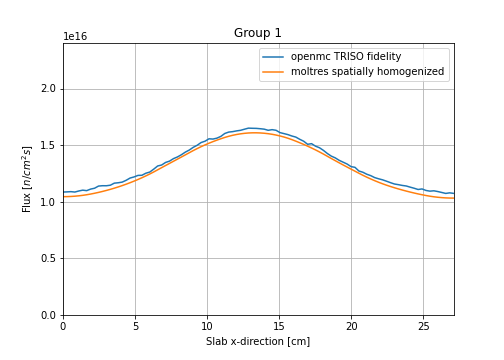
\includegraphics[width=0.48\linewidth]{flux_group1_948K.png} 
    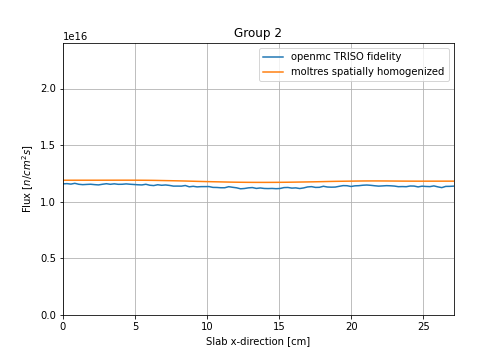
\includegraphics[width=0.48\linewidth]{flux_group2_948K.png} 
    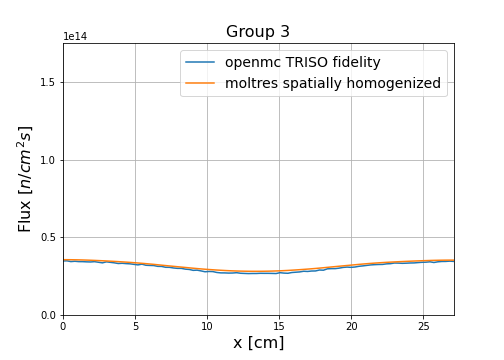
\includegraphics[width=0.48\linewidth]{flux_group3_948K.png} 
    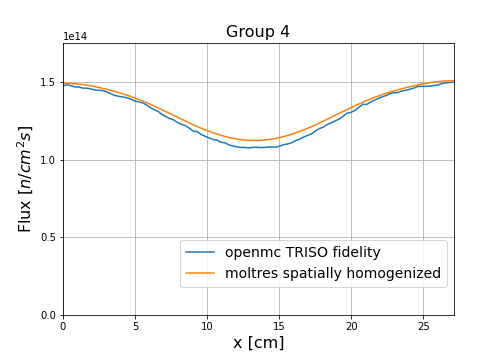
\includegraphics[width=0.48\linewidth]{flux_group4_948K.png} 
    \caption{AHTR fuel slab's centerline neutron flux distribution in 4 groups
    at 948K. 
    Energy Group 1: E $> 9.1188 \times 10^{-3}$ MeV, 
    Energy Group 2: $2.9023 \times 10^{-5} < E < 9.1188 \times 10^{-3}$ MeV,
    Energy Group 3:  $1.8556 \times 10^{-5} < E < 2.9023 \times 10^{-5}$ MeV,
    Energy Group 4:  $1.0 \times 10^{-12} < E < 1.8554 \times 10^{-6}$ MeV}
    \label{fig:flux_948K}
\end{figure}
The OpenMC simulation shows higher flux in Group 1, and lower flux in the
Group 2 and Group 3. 
However, there is an overall good agreement for each group's flux.  

\subsubsection{Neutron Energy Spectrum}
Figure \ref{fig:neutron_spectrum_948K} shows the neutron spectrum the OpenMC simulation 
for both 252 and 4 groups, and 4-group Moltres simulation. 
 \begin{figure}[]
    \centering
    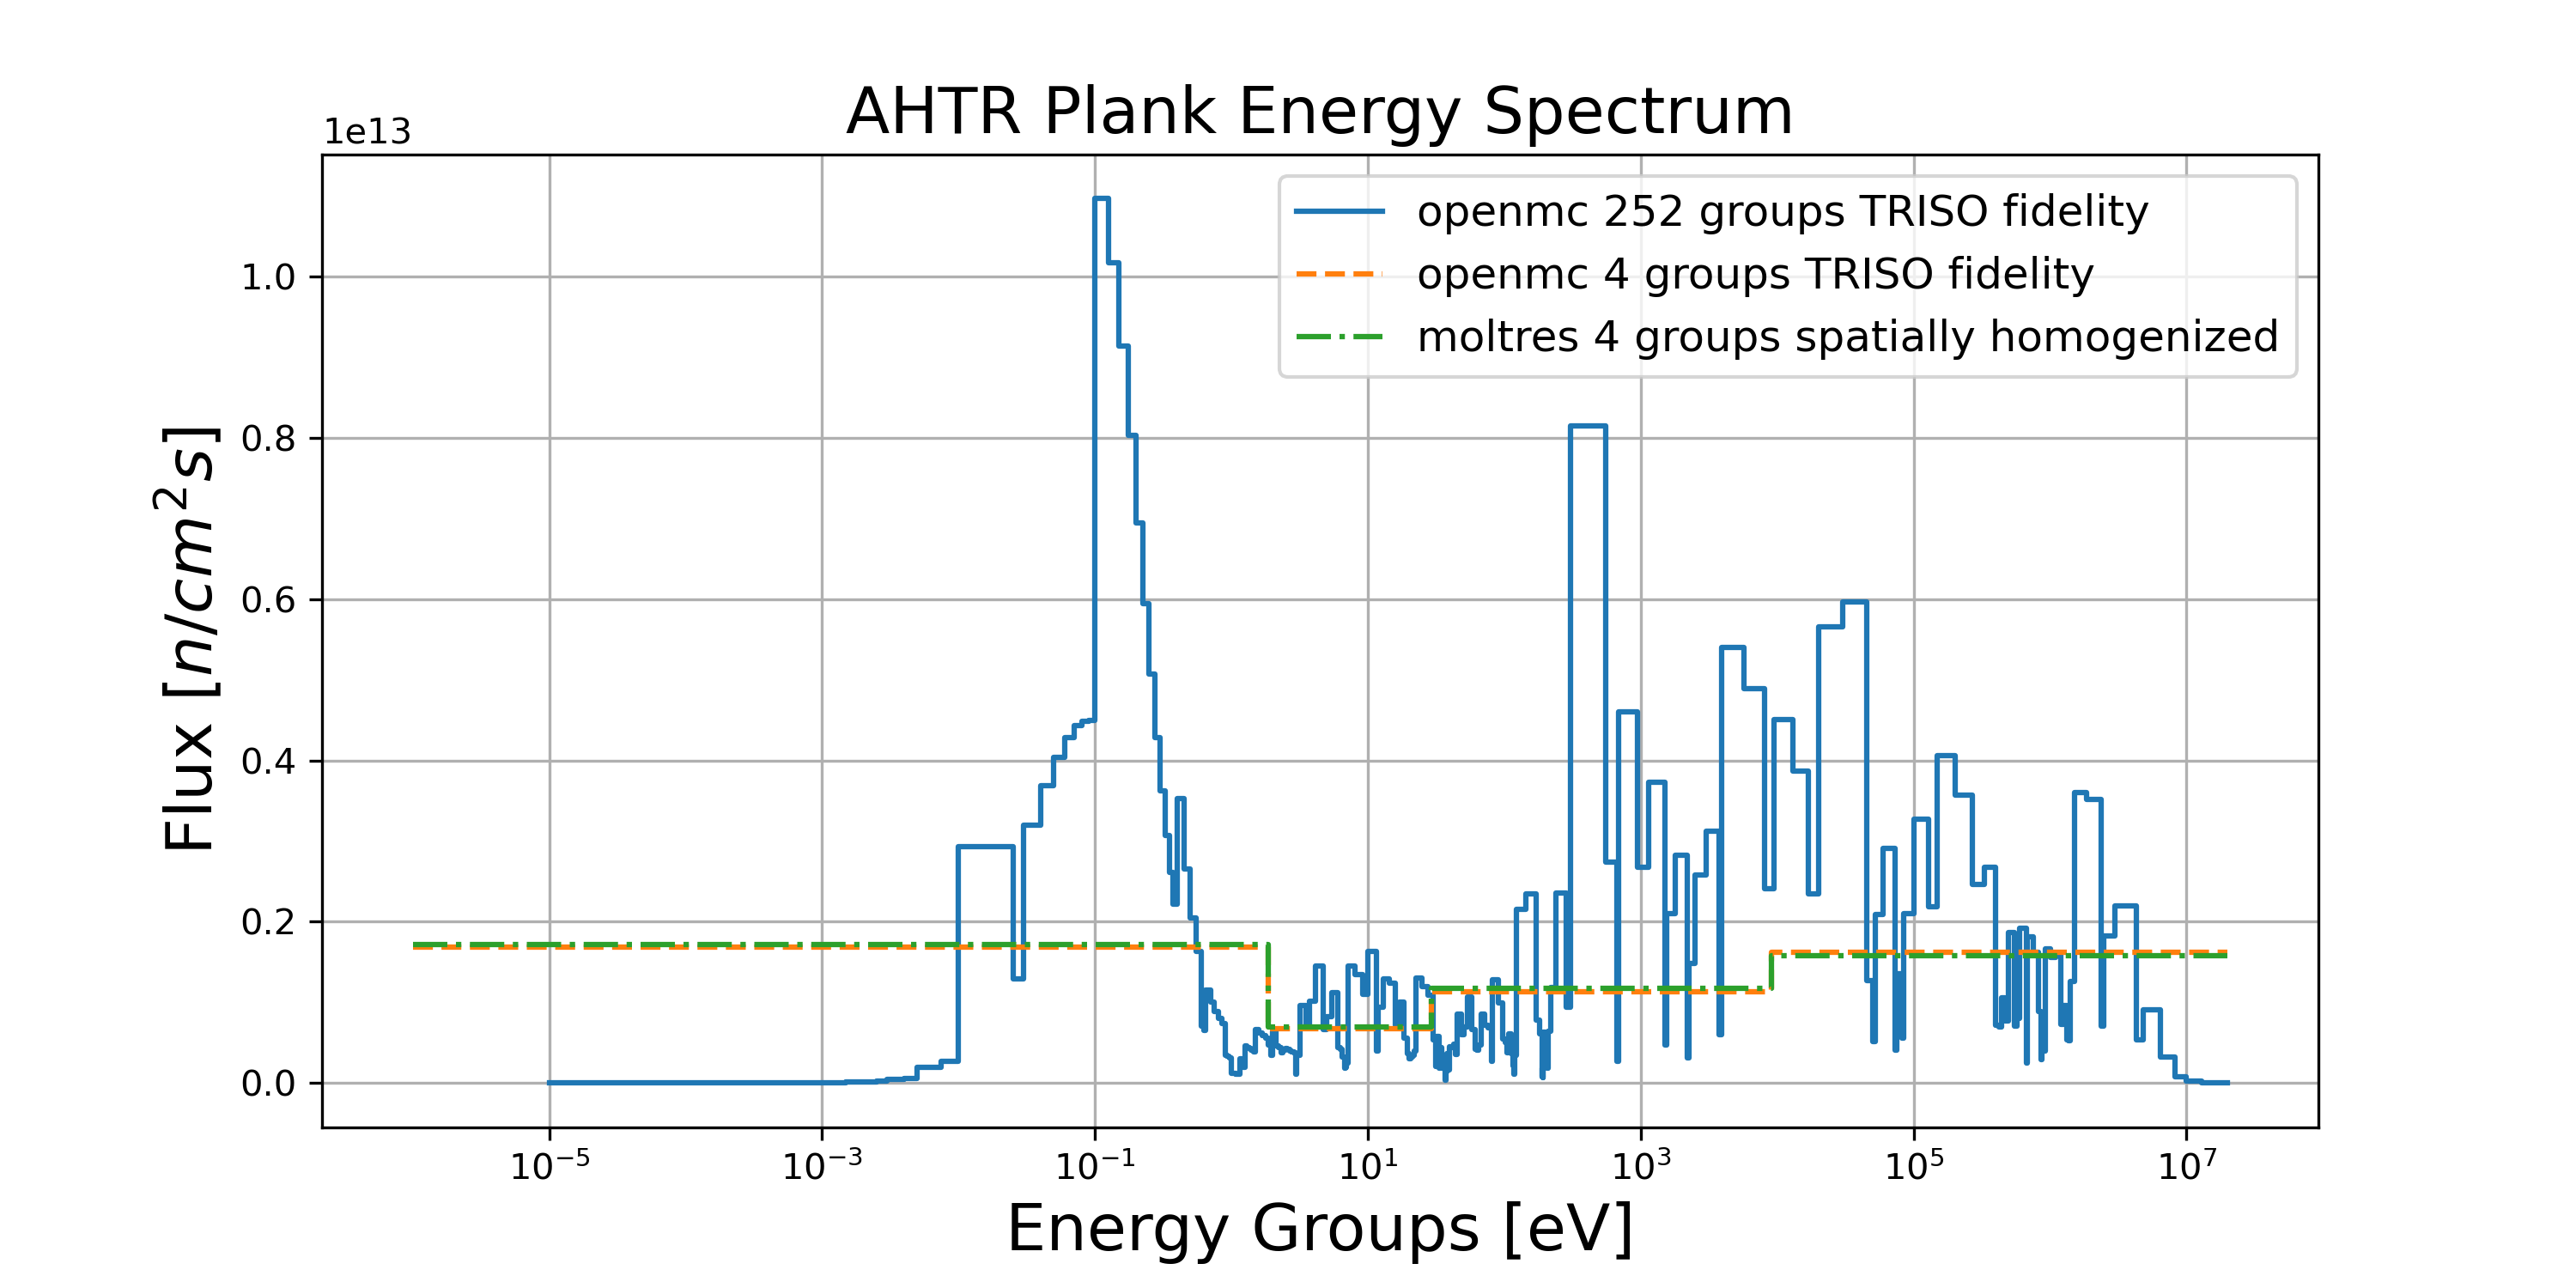
\includegraphics[width=\linewidth]{neutron_spectrum_948K.png}
    \caption{AHTR fuel slab's neutron spectrum.}  
    \label{fig:neutron_spectrum_948K}
\end{figure}
There is good agreement between OpenMC and Moltres models 4-group spectrums. 

In summary, Moltres replicated the relevant neutronics parameters accurately 
using group constant data from OpenMC for the \gls{AHTR} plank model. 

\subsection{AHTR One-Third Assembly: Key Neutronics Parameters Verification}

\subsection{AHTR Plank: Mesh Refinement Study}

\subsection{AHTR Plank: Group Constant Temperature Study}
During ROLLO optimization, each new reactor geometry results in the creation of 
a new Moltres temperature model. 
Correspondingly, a new set of group constant data will also be created. 
Group constant data for multiple temperatures requires running multiple neutronics 
simulations at the various temperatures, thus, increasing the total compute time 
required for each new reactor model. 

In this section, I explore the effects of using multiple temperature group 
constant data compared to a single temperature.
I set up Moltres AHTR steady-state temperature models for a plank (described in the 
Section \ref{sec:ahtr-moltres-temperature-model}) with group constant data at each and 
all the following temperatures: 948, 1024, 1100, and 1200 K. 
The group constant data is generated with OpenMC \gls{AHTR} models at the specified 
temperatures. 
Table \ref{tab:moltres-group-constant-temps} shows the average and maximum temperature 
reported by each Moltres model and their differences compared to the model with 
group constant data with all four temperatures. 
Table \ref{tab:moltres-group-constant-temps} also shows the 2-norm of the 
centerline temperature difference between the AHTR slab model with all four temperatures 
and each single temperature. 
\begin{table}[]
    \centering
    \onehalfspacing
    \caption{AHTR slab's average and maximum temperature and 2-norm of temperature 
    discretized across the slab's centerline for varying group constant temperature data.}
	\label{tab:moltres-group-constant-temps}
    \scriptsize
    \begin{tabular}{p{2.5cm}p{2cm}p{2.4cm}p{2cm}p{2.4cm}p{2cm}}
    \hline 
    \textbf{Group Constant Data Temps [K]}& \textbf{Ave Slab Temp [K]}& 
    \textbf{Ave Slab Temp Diff [K]}& \textbf{Max Slab Temp [K]} & 
    \textbf{Max Slab Temp Diff [K]} & $||T_{all, i} - T_{i}||$ \\ 
    \hline 
     948 & 1019.997 &  0.032 & 1128.386 &  0.080 & 0.652\\
    1024 & 1019.989 &  0.023 & 1128.640 &  0.333 & 2.279 \\
    1100 & 1019.976 &  0.011 & 1128.300 & -0.006 & 2.875 \\
    1200 & 1019.943 & -0.023 & 1128.052 & -0.255 & 4.308 \\
    All  & 1019.965 &  -     & 1128.306 & -      & -    \\
    \hline
    \end{tabular}
\end{table}
The temperature differences between the AHTR slab model with all four temperatures 
and the AHTR slab models' with each single temperature are not significant. 
The 948K single temperature group constant data has the lowest 2-norm, thus, I 
use this temperature in the neutronics model to generate the group constant data. 

\section{ROLLO Hyperparameter Tuning}